\section{Modelisation}

\subsection{A kinematic model for the car}
The first thing to take control of a system is to understand how it
works. That's what we're going to do for this car. Indeed to control
it we will have to establish these equations in order to elaborate
the commands which will be used to lead the robot. \textbf{Figure}~\ref{fig:state}
shows the cinematic equations of the car.

\begin{figure}[!ht]
    \centering
    \begin{subfigure}[b]{0.45\textwidth}
        \centering
        
            $$ f(x, u) = \left \{
            \begin{array}{c @{=} l}
                \dot{x_1}\ & \ x_4.cos(x_5) cos(x_3) \\
                \dot{x_2}\ & \ x_4.cos(x_5) sin(x_3) \\
                \dot{x_3}\ & \ \frac{x_4 sin(x_5)}{L} \\
                \dot{x_4}\ & \ u_1 \\
                \dot{x_5}\ & \ u_2 
            \end{array}
            \right. $$
        
        \caption{Equation of the car}
        \label{eqn:state}
    \end{subfigure}
    \hfill
    \begin{subfigure}[b]{0.45\textwidth}
        \centering
        \includegraphics[width=\textwidth]{Images/state_diagram.png}
        \caption{Diagram of the car}
        \label{fig:raspi_config}
    \end{subfigure}
    \caption{State equation of the car}
    \label{fig:state}
\end{figure}



In these equations $x_1$ and $x_2$ are respectively the x and y
coordinates of the robot, $x_3$ is the heading of the robot, $x_4$
represent the speed of the rear motor and $x_5$ is the steering angle
of the car controlled by the front servomotor. $L$ is the distance between
the front and the back driving shafts. In this system it is
important to identify the variables of interest. These are the variables
that we will want to control. In our case we will be interested in the 
speed of the car and its heading. \\

There is a usefully tool to use when you want to understand
how to run a system from state equations. The differential delay
graph allows you to relate the inputs to the outputs of the car.
Actually each new node represents an integration of the previous variable. There is also the link between
inputs and outputs of our system. \textbf{Figure}~\ref{fig:diff_delay}
is the differential delay graph for our car. On this graph we represented
the two variables of interest with a double circle.

\begin{figure}[!ht]
    \centering
    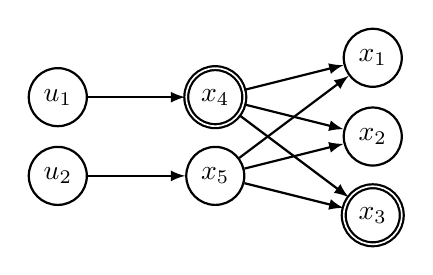
\begin{tikzpicture}[thick, scale=1, every node/.style={transform shape}]
        \tikzstyle{n}=[circle,draw]
        \tikzstyle{dn}=[circle, draw, double]
        \node[n] (U1) at (0,1) {$u_1$};
        \node[n] (U2) at (0,0) {$u_2$};
        \node[dn] (X4) at (2,1) {$x_4$};
        \node[n] (X5) at (2,0) {$x_5$};
        \node[n] (X1) at (4,1.5) {$x_1$};
        \node[n] (X2) at (4,0.5) {$x_2$};
        \node[dn] (X3) at (4,-0.5) {$x_3$};

        \tikzstyle{late}=[->,>=latex]
        \draw[late] (U1)--(X4);
        \draw[late] (U2)--(X5);
        \draw[late] (X4)--(X1);
        \draw[late] (X4)--(X2);
        \draw[late] (X4)--(X3);
        \draw[late] (X5)--(X1);
        \draw[late] (X5)--(X2);
        \draw[late] (X5)--(X3);
    \end{tikzpicture}
    \caption{Differential delay graph of our car}
    \label{fig:diff_delay}
\end{figure}

\newpage